\documentclass{article}
\usepackage{amssymb}
\usepackage{amsmath}
\usepackage{bm}
\usepackage{enumitem}
\usepackage{graphicx}
\usepackage{listings}

\title{Math 537 Final Project}
\author{Ben Anderson, Saul Hernandez, Bryan Rust}
\date{December 2024}

\begin{document}

\maketitle

\section{Introduction}
In a world optimized by automation and data, being able to interpret and understand complex, dynamic systems has become more and more crucial and beneficial in the modern world. One way to optimize and manipulate such systems is by understanding the fundamentals of discrete-time systems and control theory. 

Control theory forms the foundation of automation and electronics, helping design systems to be reliable and efficient. These mathematical theories can apply to many diverse areas from finance, to robotics such as autonomous vehicles, or healthcare, and many more. The systems monitor their environment and adjust their inputs to maintain stability, optimize performance, and respond to uncertainties.

\subsection{Discretization In Control Systems}
A significant focus in control theory is the discretization of continuous systems, enabling their implementation into digital platforms. Discrete-time systems process discrete-time signals as inputs and generate a discretized corresponding output, making these methods compatible with modern tools and systems. Discretization systems are crucial in applications that require real-time decision making such as stock market trading, automation in robotic hardware, and more, in which quick and accurate responses are needed. Through discretization, continuous-time models – which describe system behavior in infinite time resolutions – are able to be transformed  into discrete-time models, allowing for effective processing with models and controllers. This procedure ensures controllers can operate with the use of periodic updates (or feedback) rather than continuous monitoring. 

Furthermore, discretization addresses challenges in continuous-time models, like handling noise, external disruptions, and other obstacles which can hinder system stability and accuracy. By breaking continuous signals into manageable time intervals, discretization systems can improve the reliability of control systems. \cite{keles2024}


\subsection{Theoretical Application}
To optimize stability and manipulate control in time systems, discretization is typically applied to three main areas: signal processing, system modeling, and controller design. 

Discrete-time control, when applied towards signal processing, involves sampling continuous control inputs and measurements and used to create discrete-time signals. This form of discretization enables compatibility between any type of system hardware or processing framework and their relative input signals, increasing versatility and adaptability with these systems. 

Similarly, in system modeling, a discrete-time dynamic modeling system will record inputs at varying time intervals, and contribute these signals to appropriately adjust models. This discretization approach improves the interaction between input signals and digital system models, increasing the accuracy and efficiency of the representation for each control system. 

Discretization is especially effective throughout controller design, in which it enables controllers to operate alongside feedback indicators, optimizing system design and performance. By accounting for the possibility of computational delays, data sampling errors, or the possible appearance of noise in these systems, discretization enables controllers to adapt in real-time to these uncertainties and actively make adjustments. 

Ultimately, the integration of discretization in these areas optimizes the system’s functionality and performance as well as improves the system's credibility through diverse environments. \cite{keles2024}

\subsection{Practical Application}
Discretization is widely applied in real-world scenarios to monitor, regulate, and optimize data and dynamic systems. These systems are common in fields surrounding automation, management, modeling, or data analysis where systems are able to take advantage of the control and sampling of data, thus increasing productivity.

\subsubsection{Financial Analysis}
The application that will be further discussed in this paper revolves around the stock market. Here, discrete-time systems play an important role in facilitating and automating trading strategies. These systems process historical data and respond to market fluctuations at various discrete-time intervals. This gives traders the opportunity to make different data-driven decisions in real time. By using these methods to discretize continuous financial models, traders are able to utilize algorithms to break down unpredictable and complex market conditions into segments of time to maintain stability and a good performance with their models. 

For instance, high-frequency trading systems will use discrete-time systems in order to carry out thousands of trades within seconds, allowing these systems and traders to respond to any disruptions in data. These systems can also give traders the opportunity to simulate and possibly predict scenarios, utilizing trends and create models that can adjust better to disruptions.\cite{barmish2011}

\subsubsection{Other Applications}
Discretization is also practical to numerous other applications beyond financial analysis. Applying to systems related to robotics, autonomous vehicles, animation, power systems, and more. In these different discrete-time systems discretization enables the ability to control and manipulate data into more manageable time intervals.

For example, in robotics (i.e. autonomous vehicles), discrete control systems are crucial for integrating real-time interaction with varying environments. This can benefit autonomous vehicles by improving areas like navigation, avoiding obstacles, and maximizing safety relative to other vehicles on the road. These systems rely on discretized models using sensor data to make efficient adjustments to any environmental changes. 

In other applications like animation, discrete-time systems are used with motion capture systems, in which continuous motion is measured and approximated through several distinct frames. Alternatively, in power systems models are important for managing the stability of electrical grids, relying on data to distribute power to different grids and prevent possible overloads or outages. In each of these systems, discretization is used to optimize data-powered tools to maintain stability through disruptive environments.

\subsection{Research Focus \& Objectives}
This paper focuses on exploring the principles of discrete-time control systems and opportunities they open up for various applicable systems. With particular attention to uncertainties and discretization errors that come up in dynamic systems due to disruption, noise, and unpredictability. 

By introducing methods used for discretization, we aim to interpret the effectiveness towards stability and the performance of systems through real-world scenarios. Our primary application centers around financial analysis, specifically in stock markets, where discrete-time systems play a crucial role in automating trade strategies. 

Through the integration of discretization techniques and methods, this paper seeks to demonstrate how these discrete-time systems can improve and optimize accuracy, adaptability, and stability.

\section{Methods and Theory}
\subsection{Defining LTV and LTI Systems in Continuous and Discrete Time}
Discrete systems function in much the same way as continuous systems. The standard, continuous state equation can be used to form the basis of a discrete state equation. 

The LTV, or Linear Time-Variant, case of the state-space equations is implemented when the system changes with respect to time, and is valuable with the ability to adapt to feedback through the output equation. The LTV system is given by the following pair of equations:
\begin{equation}
    \dot{x(t)}=\bm{A(t)}x(t)+\bm{B(t)}u(t)
\end{equation}
\begin{equation}
    y(t)=\bm{C(t)}x+\bm{D(t)}u(t)
\end{equation}
The LTI, or Linear Time-Invariant, case of the state-space equations is a simpler framework, but this simplicity allows for more depth in analysis and allows for the use of eigenvalues for analysis and the use of transfer functions to coax out even more information from the system. The LTI system is given by the following pair of equations:
\begin{equation}
    \dot{x}=\bm{A}x+\bm{B}u
\end{equation}
\begin{equation}
    y=\bm{C}x+\bm{D}u
\end{equation}

Although these equations provide a valuable framework for modern control theory, the discrete-time implementations of these equations are just as useful, if not more, than the continuous implementations. The discrete-time state-space equations arise naturally in digital systems when time is measured discretely and in systems that rely on data sampling, which is carried out at planned discrete intervals.

These equations give the LTV case of the discrete-time state-space equations: 
\begin{equation}
    x(t+1)=\bm{A}(t)x(t)+\bm{B}(t)u(t)
\end{equation}
\begin{equation}
    y(t) = \bm{C(t)}x+\bm{D(t)}u(t)
\end{equation}

These equations give the LTI case of the discrete-time state-space equations:
\begin{equation}
    x^{+}=\bm{A}x+\bm{B}u
\end{equation}
\begin{equation}
    y=\bm{C}x+\bm{D}u
\end{equation}

\subsection{Solutions to the State-Space Equation}
For the first discussion of solutions to these systems of equations, we know that the solution to the LTV system is given by 
\begin{equation}
    x(t)=\Phi(t,t_0)x_0+\int_{t_0}^{t} \Phi(t,\tau)\bm{B}(\tau)u(\tau)d\tau
\end{equation}
 
 From this equation we are able to compute the discrete time solution to the equation which is given as the piecewise defined function:
\begin{equation}
    x(t)=\Phi(t,t_0)x_0,
\end{equation}
\begin{align}
    \Phi(t,t_0)=
    \begin{cases}
        \bm{I};\qquad t=t_0 \\
        \bm{A}(t-1)\bm{A}(t-2)...\bm{A}(t_0+1)\bm{A}(t_0); \qquad t>t_0
    \end{cases}
\end{align}

In the same matter, since we know that the solution to the LTI system is given by
\begin{equation}
    x(t)=e^{\bm{A}(t-t_0)}x_0+\int_{t_0}^{t} e^{\bm{A}(t-\tau)}\bm{B}u(\tau)d\tau
\end{equation}

Noting that in discrete-time integration is functionally replaced by summation, we are able to derive the solution in the discrete-time case 
\begin{equation}
    x(t) = A^{t - t_0} x_0 + \sum_{\tau = t_0}^{t-1} A^{t-1-\tau} B u(\tau)
\end{equation}

\subsection{Zero-Order Hold Discretization}
One well known method of discretizing an LTI system is the zero-order hold, or ZOH. This method is loosely similar to a Riemann sum as it uses steps where the value is "held" constant over a given interval. The ZOH is computationally simple compared to many other discretization methods and is widely used in any digital-to-analog conversions. The ZOH uses the equations (1) and (2) and converts them into discrete-time piecewise-stepped functions through the iterative definition:
\begin{equation}
    x_{k+1}=\bm{A}_dx_k+\bm{B}_du_k
\end{equation}
where $\bm{A}_d$ and $\bm{B}_d$ are defined as:
\begin{equation}
    \bm{A}_d=e^{\bm{A}T}
\end{equation}
\begin{equation}
    \bm{B}_d=\int_{0}^{T} e^{\bm{A}\tau}\bm{B}d\tau
\end{equation}
Further, since we know when $\bm{A}$ is invertible, we can use the fact:
\begin{equation}
    \int_{0}^{T}e^{\bm{A}\tau}d\tau = \bm{A}^{-1}(e^{\bm{A}T}-\bm{I})
\end{equation}
$\bm{B}_d$ can be represented as:
\begin{equation}
    \bm{B}_d=\int_{0}^{T} e^{\bm{A}\tau}\bm{B}d\tau=\bm{B}\int_{0}^{T} e^{\bm{A}\tau}d\tau=\bm{A}^{-1}(e^{\bm{A}T}-\bm{I})\bm{B}
\end{equation}

These equations are effective at discretizing the continuous-time LTI system, however, like the Riemann sums that this method is reminiscent of, the ZOH is an approximation of the original system where the input of the system is forced to remain constant over the interval $[kT, (k+1)T)$ rather than following the actual input of the system from the true, continuous-time LTI system.

The biggest shortcoming of the ZOH is the accuracy of the approximation, however, to compensate for this one can use first-order holds, which uses linearity to provide a more accurate approximation of the LTI system. Further, there are also second-order holds and higher-order than that, which increase accuracy even further at the expense of computational cost. We will not be covering these as they are used primarily in signal reconstruction which is outside the scope of this paper. 

\subsection{2x2 case of the Zero-Order Hold Discretization}
To give an example of this, take the 2x2 case of the LTI system with the matrix $\bm{A}=$
$\begin{bmatrix}
    a_{11} & a_{12} \\
    a_{21} & a_{22}
\end{bmatrix}$
and the matrix $\bm{B}=$
$\begin{bmatrix}
    b_{11} \\
    b_{12}
\end{bmatrix}$.

These matrices give us the following LTI system:
\begin{equation}
    \dot{x}=
    \begin{bmatrix}
    a_{11} & a_{12} \\
    a_{21} & a_{22}
    \end{bmatrix}x+
    \begin{bmatrix}
    b_{11} \\
    b_{12}
    \end{bmatrix}u
\end{equation}

We can apply the ZOH to this system by defining $\bm{A}_d$ and $\bm{B}_d$ as:
\begin{equation}
    \bm{A}_d=e^{
    \begin{bmatrix}
    a_{11} & a_{12} \\
    a_{21} & a_{22}
    \end{bmatrix}T}
\end{equation}
\begin{equation}
    \bm{B}_d=\int_{0}^{T}e^{
    \begin{bmatrix}
    a_{11} & a_{12} \\
    a_{21} & a_{22}
    \end{bmatrix}\tau}
    \begin{bmatrix}
    b_{11} \\
    b_{12}
    \end{bmatrix}d\tau
\end{equation}


Combining these equations, we can generalize the ZOH discretization of the LTI system, equation (19), in a way that will hold for any 2x2 LTI system as:
\begin{equation}
    x_{k+1}=e^{
    \begin{bmatrix}
    a_{11} & a_{12} \\
    a_{21} & a_{22}
    \end{bmatrix}T}x_k+\int_{0}^{T}e^{
    \begin{bmatrix}
    a_{11} & a_{12} \\
    a_{21} & a_{22}
    \end{bmatrix}\tau}
    \begin{bmatrix}
    b_{11} \\
    b_{12}
    \end{bmatrix}d\tau u_k
\end{equation}

Further, if we assume that the matrix $\bm{A}$ is invertible so that we can guarantee that $\bm{A}^{-1}$ exists, we can eliminate the integral and further simplify $\bm{B}_d$ to:
\begin{equation}
    \bm{B}_d=\frac{1}{a_{11}a_{22}-a_{12}a_{21}}
    \begin{bmatrix}
        a_{22} & -a_{12} \\
        -a_{21} & a_{11}
    \end{bmatrix}
    (e^{
    \begin{bmatrix}
    a_{11} & a_{12} \\
    a_{21} & a_{22}
    \end{bmatrix}T}-
    \begin{bmatrix}
        1 & 0 \\
        0 & 1
    \end{bmatrix})
    \begin{bmatrix}
         b_{11} \\
        b_{12}
    \end{bmatrix}
\end{equation}

This results in the following ZOH equation:
\begin{equation}
    x_{k+1}=e^{
    \begin{bmatrix}
    a_{11} & a_{12} \\
    a_{21} & a_{22}
    \end{bmatrix}T}x_k+\frac{
    \begin{bmatrix}
        a_{22} & -a_{12} \\
        -a_{21} & a_{11}
    \end{bmatrix}
    (e^{
    \begin{bmatrix}
    a_{11} & a_{12} \\
    a_{21} & a_{22}
    \end{bmatrix}T}-
    \begin{bmatrix}
        1 & 0 \\
        0 & 1
    \end{bmatrix})
    \begin{bmatrix}
         b_{11} \\
        b_{12}
    \end{bmatrix}}{a_{11}a_{22}-a_{12}a_{21}}u_k
\end{equation}

This equation can be further simplified by applying the matrix exponential to the matrix $e^{\bm{A}T}$, however without loss of generality, we will not simplify since the structure of the matrix in not precisely known. 

\subsection{The Mixed Method}
Another approach to discretizing LTI systems that was first explored recently is called the Mixed Method. It should be noted that the authors recognize that the matrices $\bm{A}$ and $\bm{B}$ are not necessarily known, apart from the fact that they share dimensions. This method defines steps forward in time with the recursive relationship given below. \cite{keles2024}
\begin{equation}
    t_k = t_{k-1} + \Delta t
\end{equation}
Using the notation put forward in the paper, we see that this method applies the solution to the LTI system described above, but with different weights of importance on the different time steps given by $\alpha_s$, where it is important to note that $s=1,2,...,N$.

The first step is given by:
\begin{equation}
    x_k=e^{\bm{A}_{\lambda}(t_k(t_k-\Delta t))}x_{k-1}+\int_{t_k-\Delta t}^{t_k}e^{\bm{A}_{\lambda}((t_k-\tau))}\bm{B}_\lambda u(\tau)ds
\end{equation}

And more generally, for the $N^{th}$ iteration of the method:
\begin{equation}
    x_k=e^{\bm{A}_{\lambda}(t_k(t_k-N\Delta t))}x_{k-N}+\int_{t_k-N\Delta t}^{t_k}e^{\bm{A}_{\lambda}((t_k-\tau))}\bm{B}_\lambda u(\tau)ds
\end{equation}
Now implementing the $\alpha$ into weighting of these solutions to add different delays which is given by the equation:
\begin{equation}
    x_k=\sum_{s=1}^{N} \alpha_s e^{\bm{A}_\lambda s \Delta t}x_{k-s} + \sum_{s=1}^{N} \alpha_s \int_{t_k -s \Delta t}^{t_k} e^{\bm{A}_\lambda (t-\tau)}\bm{B}_\lambda u(\tau) d(\tau)
\end{equation}
This method, although computationally intensive, uses this multistep methodology that, with optimization tailored to the specific system in question, can minimize errors in the discretization process, allowing for a more accurate control measure on the system.

This methodology is useful in the discussion of sampled-data control, where the feedback and system control is driven by sampling at discrete intervals. The multistep approach found within the Mixed Method allows for a more precise control from measured systems.

\section{Results}
To demonstrate the discrete-time system methodologies, we applied the Zero-Order Hold and Mixed Method discretization techniques to a stock market trading strategy. 

This application highlights how discretization methods can improve system performance, mitigate of errors, and enhance stability in financial decision-making under uncertain and diverse conditions.

\subsection{Stock Market Trading Strategy}
We developed a sampled model to predict asset prices and execute trades based on discrete intervals. The system relied on historical price data as state inputs and applied the Zero-Order Hold Discretization \& Mixed Method to discretize the continuous-time financial models, enabling access to optimized trade decisions at specific time intervals.

\subsection{Setup}
\begin{itemize}
    \item \textbf{Data:} We created a simulated stock price data for an asset, sampled over different periods in a controlled environment

    Data was generated using a sine function, creating predictable price changes to be able to effectively compare the two methods. This enabled the ability to evaluate the performance of both methods through different price changes. Providing a simpler data sample, leading to an understandable analysis.
    \item \textbf{Parameters:} Sampling intervals were set at 1, 5, and 15 minutes to simulate different trading frequencies, reflecting low, moderate, and high trading scenarios
    
    \item \textbf{Metrics:} To evaluate performance of each discretization method, we considered the accuracy of predictions, representation of profit margins over time, and the stability of each system through sudden and diverse market fluctuations.
    
\end{itemize}

\subsection{Methods}
\begin{enumerate}
    \item \textbf{Discretization:} The continuous-time price prediction models were discretized using both the Zero-Order Hold and the Mixed Method.
    \begin{itemize}
        \item \textbf{ZOH:} Treated the input as constant over each interval. [Figure \ref{fig:zohmm1}]
        \begin{figure}
            \centering
            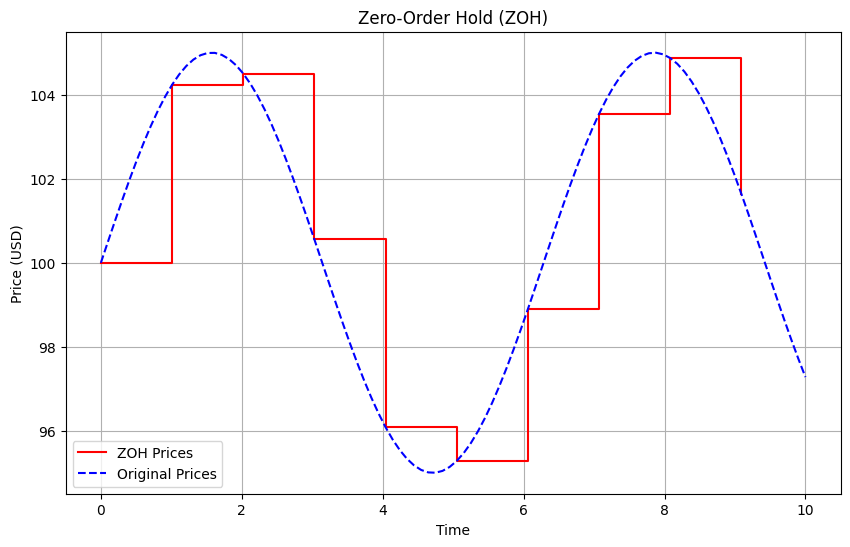
\includegraphics[width=0.55\linewidth]{ZOH.png}
            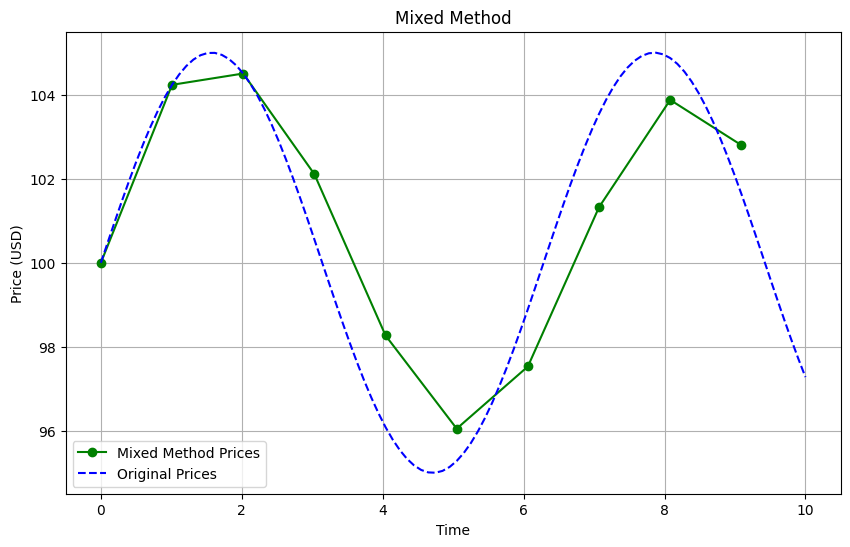
\includegraphics[width=0.55\linewidth]{MM.png}
            \label{fig:zohmm1}
        \end{figure}
        \item \textbf{Mixed Method:} Incorporated multiple past time steps with optimized weights ($\alpha$ coeffs) to capture market trends. [Figure \ref{fig:zohmm1}]
    \end{itemize}
    \item \textbf{Trade Execution:} A simple rule-based trading strategy was used, where buy and sell decisions were made based on predicted price changes.
    \begin{itemize}
        \item \textbf{Buy Signal:} When predicted it will rise
        \item \textbf{Sell Signal:} When predicted it will lower
    \end{itemize}
\end{enumerate}

\subsection{Findings}
\begin{enumerate}
\item Prediction Accuracy:
    \begin{itemize}
        \item To compare the methods we used a  simulated stock price at sampling intervals of 1, 10, and 20 minute time steps. The Mixed Method achieved a lower error in price prediction compared to ZOH, especially at longer sampling intervals. [Figure \ref{fig:zohmm2}]
    \end{itemize}
\item Profit Margins:
    \begin{itemize}
        \item Trades executed using the Mixed Method will yield a higher average profit compared to ZOH-based strategies, gaining a more reliable prediction.
            \begin{enumerate}[label=\roman*.]
                \item \textbf{1 Minute Intervals:} Potential to give higher profits, although it has frequent buy and sell actions resulting in  more transaction costs
                \item \textbf{10 Minute Intervals:} Balanced performance with medium trade frequency
                \item \textbf{20 Minute Intervals:} A lot less trades which result in low transaction costs, though you will have less responsiveness
            \end{enumerate}
    \end{itemize}
\item System Stability:
    \begin{itemize}
        \item The Mixed Method demonstrates a  greater flexibility during longer periods, avoiding losses that can happen in the ZOH-based approach
    \end{itemize}
\item Computational Cost:
    \begin{itemize}
        \item Although the Mixed Method uses more computation time, its potential profit with more accurate predictions balances it out. 
    \end{itemize}
\end{enumerate}
\begin{figure}
    \centering
    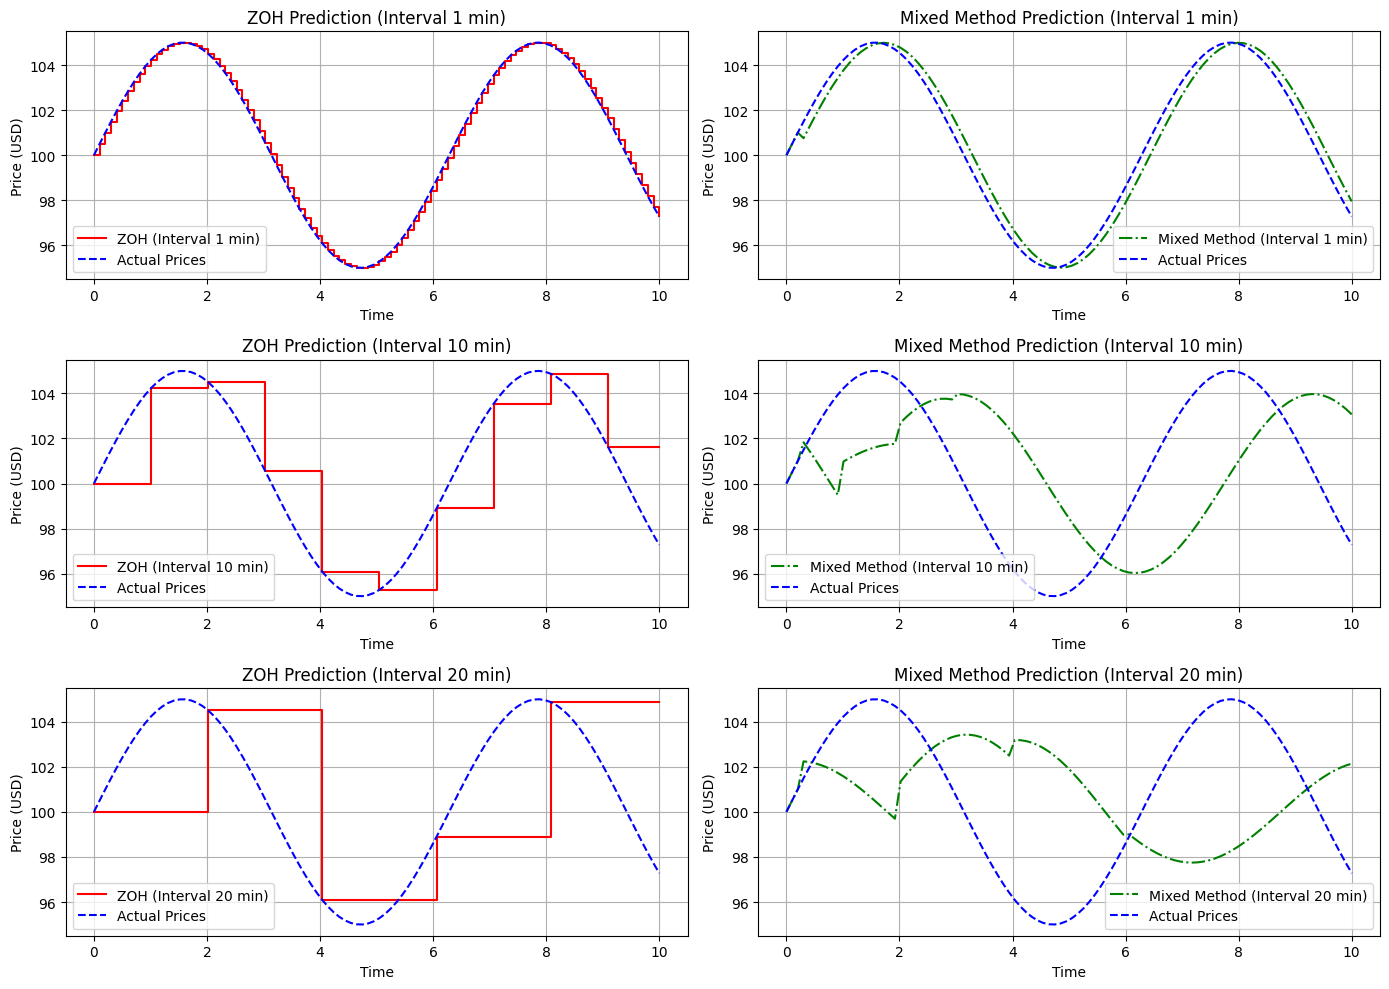
\includegraphics[width=1\linewidth]{zoh_mm.png}
    \label{fig:zohmm2}
\end{figure}

\subsection{Analysis}
The results show that ZOH has minimal computation and can be effective when prices are stable. While the Mixed Method has more accurate predictions with fluctuations in the market – offering more potential profits. 

Overall, we see that the shorter the intervals, the better the predictions will be, but it will incur a higher cost from frequent trading. Therefore, the method can support trading strategies that allow more flexible and profitable trading in the markets.


\section{Discussion \& Summary}

\subsection{Discussion}
In this project, we studied discretization applications in stock market trading. The two methods we used were the Zero-Hold Method and the Mixed Method. The goal was to see how each method affects the predicted price of the simulated stock more accurately, their stability, and the profit they can potentially offer. 

From the results, we see that the discretization method Zero-Order Hold is only efficient when the prices of the stock are stable, and the Mixed Method gives a better prediction, especially in a fluctuating price. It also worked better in longer time intervals because it uses previous time steps which helps better understand market trends. Thus we can say that the Mixed Method outperformed ZOH in these terms.

In regards to profits, the Mixed method performed better as time intervals got longer, leading to higher returns such as more possible gains and fewer possible losses. Even though the ZOH was useful in stable markets, when the market became more unpredictable and time intervals got longer, it clearly struggled (fewer profits / more losses). However, when we applied the Mixed Method, it maintained more reliability at said struggles. In addition, while the method demands more computations, the accuracy of prediction and the potential gains make the trade-off worth its cost.

As the stock market is very volatile, it is important to keep stability in mind. As shown in the results, we see that the Mixed Method responded better to fluctuations in the price. Showing that it is less likely to experience a loss than the ZOH method – the Zero-Order approach struggled more to adjust to rapid changes.  
In general, the Mixed Method’s accuracy and stability offer better returns in an unstable environment than the Zero-Order Hold. Despite its computational demand, the balance of its performance offers a good choice for price predictions which can be helpful with fast decision-making for traders. 

\subsection{Conclusion}

Discrete-time systems, fundamental to control theory, play a significant role in optimization with various data-drive fields. Fields like financial market analysis, robotics, power, and more are improved through discretization. With discrete-time systems, these fields are able to improve areas like system stability, performance, and flexibility through diverse environments, addressing different challenges continuous-time systems might encounter, like noise and external disruptions.

This research demonstrated the applicability of discretization in stock market trading in order to optimize strategies. The paper focused on the two methods, Zero-Order Hold and the Mixed Method to discretize financial continuous-time models into discrete time intervals. Finding that the Mixed Method provides higher stability in sudden price changes and better predictions, resulting in better profit margins. These advantages show optimal use despite the opportunity cost of high computation, giving traders a balanced trade-off. 

To conclude, while both techniques have their strengths, the accuracy and stability of the Mixed Method stand out, specifically in longer time intervals, where it performs well in market diversity. Future research can focus on further developing these methods to handle higher degrees of data diversity and unpredictability.


\section{Appendix}

\subsection{Code Used (Python)}
\begin{lstlisting}
import numpy as np
import matplotlib.pyplot as plt

# Simulated Data
time = np.linspace(0, 10, 100)
prices = 100 + 5 * np.sin(time)  # Example price movement

# ZOH
sampling_interval = 10
zoh_time = time[::sampling_interval]
zoh_prices = prices[::sampling_interval]

# Mixed Method (Weighted Average)
mixed_weights = [0.6, 0.3, 0.1]
mixed_prices = []
for i in range(len(zoh_prices)):
    if i < len(mixed_weights):
        mixed_prices.append(zoh_prices[i])
    else:
        weighted_avg = sum(mixed_weights[j] * zoh_prices[i - j] for j in 
        range(len(mixed_weights)))
        mixed_prices.append(weighted_avg)

# Plot ZOH
plt.figure(figsize=(10, 6))
plt.step(zoh_time, zoh_prices, where='post', label='ZOH Prices', color='r')
plt.plot(time, prices, label='Original Prices', color='b', linestyle='--')
plt.title('Zero-Order Hold (ZOH)')
plt.xlabel('Time')
plt.ylabel('Price (USD)')
plt.legend()
plt.grid(True)
plt.show()

# Plot Mixed Method
plt.figure(figsize=(10, 6))
plt.plot(zoh_time, mixed_prices, label='Mixed Method Prices', color='g', 
marker='o')
plt.plot(time, prices, label='Original Prices', color='b', linestyle='--')
plt.title('Mixed Method')
plt.xlabel('Time')
plt.ylabel('Price (USD)')
plt.legend()
plt.grid(True)
plt.show()

# Prediction Functions
def ZOH(prices, sampling_interval):
    zoh_predict = np.repeat(prices[::sampling_interval], sampling_interval)
    return zoh_predict[:len(prices)]

def mixed_meth(prices, sampling_interval, weights):
    mixed_predict = []
    for i in range(len(prices)):
        if i < len(weights):
            mixed_predict.append(prices[i])
        else:
            weighted_sum = sum(weights[j] * prices[i - (j + 1) * 
            sampling_interval] for j in range(len(weights)))
            mixed_predict.append(weighted_sum)
    return np.array(mixed_predict)

# Parameters
sampling_intervals = [1, 10, 20]
weights = [0.6, 0.3, 0.1]
\end{lstlisting}

Based off of code from \cite{kantor2024}

\section{Representation in STEM}
In the many different fields that can fall under the umbrella of STEM, minorities have been historically underrepresented. This lack of equity within STEM has led to a field that has long been one sided within the workforce and schooling. With more equitable representation and inclusion in STEM fields, these fields will only grow and enhance innovations.

\subsection{Demographics and Representation in the Workplace}

In STEM fields, as of 2019, women made up approximately 52\% of all workers, which, based off of 2020 census data, is over 60,000 women in the workforce. However, when this figure is compare to STEM occupations, this number drops significantly. From the same data, only 12,000 workers in STEM fields were women, which is only 34\% of the workforce in STEM fields. There is an increase of women in STEM between 2010 (from the same data from the previous census) and 2019 however that change is accompanied by a similar increase of women working in non-STEM fields, implying that the change in STEM fields was a result of an increase in the population of women in the workforce.\cite{stem2023}\cite{census2020}

There has been a long, documented underrepresentation of many races and ethnicities. To put things into perspective, the total workforce is comprised of 61\% white, 18\% Hispanic or Latino, 12\% black or African American, 6\% Asian, which these percentages match almost exactly to the overall population data from the 2020 census. In STEM fields, the percentages differ. The percentage of white workers increases to 65\% and the percent of Asian workers increases to 9\%. However, the percentage of Hispanic or Latino and Black or African American workers in STEM drops to 14\% and 8\% respectively. This drop in percentage for these groups highlights the deep, underlying underrepresentation in STEM fields. While we see these trends in STEM fields, we see exactly the inverse  trends in non-STEM fields among all racial and ethnic groups.\cite{stem2023}\cite{census2020}
\subsection{Demographics and Representation at SDSU}

While by no means is the data for enrollment and socioeconomic makeup of SDSU extend to colleges and universities as a whole, the data here is important to understand as a part of the SDSU community. As of the fall 2024 semester, the College of Engineering and the College of Engineering have a combined enrollment of 10,390 across all majors and between undergraduate and graduate students. Note the data only includes full-time students.\cite{enrollment2024}

In the enrollment data, we see that between all levels and majors in these two colleges, the have a more equal composition by sex. In total 4,816 students enrolled are women. This is over 46\% of STEM students at SDSU. However the total enrollment for the two colleges can be deceiving as we see that in all programs except for Psychology loosely follow the same demographic trends that we saw in the STEM workforce. In the psychology program, which numbers 2,375 students makes up nearly a quarter of the enrollment in two STEM colleges combined, the enrollment is nearly 82\% women. This is a massive number and the statistical outlier from the rest of the enrollment data for STEM programs at SDSU.
At SDSU the racial and ethnic enrollment also differs from the national workplace composition. If we take that to be the baseline, we can notice large scale differences in the percentage of ethnicities represented in the data. The biggest changes from the national work sampling is white, which makes up less than a third of all STEM students at SDSU, a drop of over 30\% of from the national workplace data, and Hispanic or Latino students, who make up over 32\% of the STEM students, interestingly enough the percentages for these two groups is the same. However, for Black or African Americans the percentage is merely 3\%, a sharp drop from the workplace data.\cite{enrollment2024}\cite{stem2023}

\subsection{Consequences of Inequitable Representation in STEM}

One common application that combines disciplines from across STEM is AI. Since AI expands its capabilities through machine learning and large language models through word embedding. The The mathematical clusters that are formed through the embedding perpetuate inequalities by clustering different words together. One example of this is, due to the majority of STEM workers being men, that men are more closely correlated to words like 'math' or 'engineer' while women were correlated more to homemaking or the arts. The AI model perpetuated the idea of men as the scientists and women as homemakers because of the lack of representation of women in fields like STEM illustrating the need for more thought to be put into inclusion of women in STEM and the data AI is trained on. \cite{devlin2017}

A second, deeply troubling, word flower correlation that AI has learned is grouping  names of African Americans, rather than European Americans, closer to other objects and ideas with more negative connotations whereas European American names were much more closely related to words like 'gift' and 'happy' in the database. As of just 2023, after image recognition software has mislabeled people who are Black as gorillas, which brings up historical, racist language because these models had not been well trained. These AI models had not been trained on a diverse set of images of people. These examples highlight the lack of diverse representation and equitable standings within the STEM community. AI models highlight and bring forward problems and systematic biases that is found within the data that they are trained on. \cite{devlin2017}\cite{grant2023}

AI is but one example where a lack of diversity and equitable representation across sex, race, and ethnicity shows the systematic issues that are faced today. It is an example that is becoming more and more present as AI, especially chat bot AI, is becoming more commonplace in everyday life. The historical problems that AI has had show the underlying issues that are faced within the entire STEM community, "This is showing that we're prejudiced and that AI is learning it."\cite{devlin2017} AI highlights the need to build a more diverse and inclusive environment, which if STEM workplace demographics and SDSU enrollment data can be taken as a sample, shows that, over the last fifteen years, many steps have been taken towards this goal, but there are many more steps to walk on this path.

\begin{thebibliography}{9}

\bibitem{barmish2011}
    B. R. Barmish, 
    \textquotedblleft On performance limits of feedback control-based stock trading strategies,\textquotedblright 
    Proceedings of the 2011 American Control Conference, San Francisco, CA, USA, 2011, pp. 3874-3879, doi: \texttt{10.1109/ACC.2011.5990879}.
    Keywords: Investments; Mathematical model; Equations; Feedback control; Differential equations; Economic indicators; Adaptive control.

\bibitem{keles2024}
    Natalia Augusto Keles, et al. 
    \textit{Discretization and State Feedback Control for Uncertain Linear Systems}. 
    Journal of the Franklin Institute, vol. 361, 2024. 
    Available at: \texttt{https://doi.org/10.1016/j.jfranklin.2023.12.006}.

\bibitem{enrollment2024}
    \textit{Enrollment Data}. 
    Available at: \texttt{https://asir.sdsu.edu/enrollment-data/}.

\bibitem{stem2023}
    \textit{The STEM Labor Force of Today}. 
    National Science Foundation. 
    Available at: \texttt{https://ncses.nsf.gov/pubs/nsb20212/participation-of-demographic-groups-in-stem}.

\bibitem{census2020}
    \textit{2020 Census Demographic Profile}. 
    United States Census Bureau. 
    Available at: \texttt{https://www.census.gov/data/tables/2023/dec/2020-census-demographic-profile.html}.

\bibitem{devlin2017}
    Hannah Devlin. 
    \textit{AI programs exhibit racial and gender biases, research shows}. 
    2017. 
    Available at: \texttt{https://www.theguardian.com/technology/2017/apr/13/ai-programs-exhibit-racist-
    and-sexist-biases-research-reveals}.

\bibitem{grant2023}
    Grant and Hill. 
    \textit{Google’s photo app still can’t find gorillas. And neither can Apple’s}. 
    2023. 
    Available at: \texttt{https://ekathimerini.com/nytimes/1212118/googles-photo-app-still-cant-find-gorillas
    -and-neither-can-apples/}.

\bibitem{kantor2024}
    J. C. Kantor. 
    \textit{Zero-Order Hold and Interpolation}. 
    Available at: \texttt{https://jckantor.github.io/CBE30338/08.01-Zero-Order-Hold-and-Interpolation.html}.
\end{thebibliography}

\end{document}